\newpage
\begin{center}
  \textbf{\large АННОТАЦИЯ}
\end{center}

В настоящей работе рассматриваются белковые комплексы вида белок-белок, где в качестве компонент комплекса выступают белки, представленные в полноатомном виде. При моделировании процесса образования устойчивого комплекса компонентами при их нековалентном взаимодействии друг с~другом возникает необходимость в~вычислении энергии такого взаимодействия. Одним из существующих методов для вычисления энергии взаимодействия является использование оценочной функции, которая для заданной пространственной конфигурации компонент позволяет приближенно оценить искомую энергию. В~исследовании приведено описание разработанной оценочной функции, в~которой учитываются силы межатомных взаимодействий, представленные эмпирическими потенциалами Кулона и Леннард-Джонса. Молекулы растворителя в~явном виде не рассматриваются, для этого энергия сольватации вычисляется в~рамках модели неявного растворителя. При помощи k-d-дерева произведена оптимизация этапа поиска взаимодействующих атомов между различными компонентами комплекса. Для тестового набора комплексов приведены результаты применения оценочной функции, которые показывают приемлемый уровень корреляции выполняемых оценок при сравнении с~существующими инструментами. В~различных численных экспериментах продемонстрированы результаты оптимизации оценочной функции, которые демонстрируют уменьшение времени выполнения оценки энергии взаимодействия. \\


In this work protein-protein complexes considered in full-atom form and consists of several components. Protein-protein complex component assembly is guided by the establishment of non-covalent interactions. To estimate the strength of such interactions at different steps of binding score functions are usually used. In this study presented score function that estimate energy for the given spatial configuration of the protein subunits in complex. Score function considers interatomic interactions through Coulomb and Lennard-Jones potentials. Solvent molecules are not considered explicitly. The implicit solvent model is used to calculate solvation energy. The k-d-tree was used to optimize the search for interacting atoms between different components of the complex. The result of using score fucntion on the test set of protein-protein complexes is presented. It demonstrates an acceptable level of correlation compared to existing tools. The work presents results of various numerical experiments for a test set of different protein-protein complexes which demonstrates an acceptable decrease in~the time of score evaluation in comparision with other score instruments.

\onehalfspacing
\thispagestyle{empty} 

\newpage
\renewcommand{\contentsname}{\centerline{\large СОДЕРЖАНИЕ}}
\setcounter{page}{4}
\tableofcontents

\newpage
\begin{center}
  \textbf{\large ВВЕДЕНИЕ}
\end{center}
\addcontentsline{toc}{chapter}{ВВЕДЕНИЕ}

Функцию для оценки энергии взаимодействия лиганда с белком в заданной пространственной конфигурации называют <<оценочной функцией>> (\textit{scoring function})~\cite{lizunov}. В настоящее время разработано множество оценочных функций, которые подразделяются на группы, исходя из принципов их построения. Например, распространено нестрогое деление на эмпирические, статистические и функции на основе силовых полей~\cite{ci500731a}. Помимо точности оценки искомой энергии взаимодействия важными критерием выбора оценочной функции является вычислительная сложность процедуры оценки, поэтому при моделировании взаимодействия на больших временных масштабах прибегают к моделям с упрощенным представлением белков~\cite{biom10071056}, а также исключают конформационную подвижность, рассматривая компоненты комплекса как <<твёрдые>> тела, совершающие в растворителе только поступательные и вращательные движения.

Целями работы являются: разработка, реализация, оптимизация и~верификация оценочной функции для учета межмолекулярных взаимодействий в~белковых комплекса в~рамках библиотеки для полноатомного моделирования белковых комплексов PSM~\cite{psm} (\textit{protein structure modeling}). Разработка библиотеки PSM проходит в~рамках НИР в~университете <<Дубна>>, которая позволяет моделировать процесс образования белкового комплекса с~помощью кинетического метода Монте-Карло\cite{Voter}. В~основе метода лежит классическая теория переходного состояния, где в~процессе моделирования система движется в~сторону наименьшей полной энергии по пути с~наименьшими энергетическими барьерами, что позволяет модельной системе на пути к~термодинамическому равновесию проходить через последовательность квазиравновесных состояний. На определенном этапе метода требуется выполнить оценку взаимодействия, как представлено на рис.~\ref{monte}. 

\begin{figure}[h!]
	\centering
	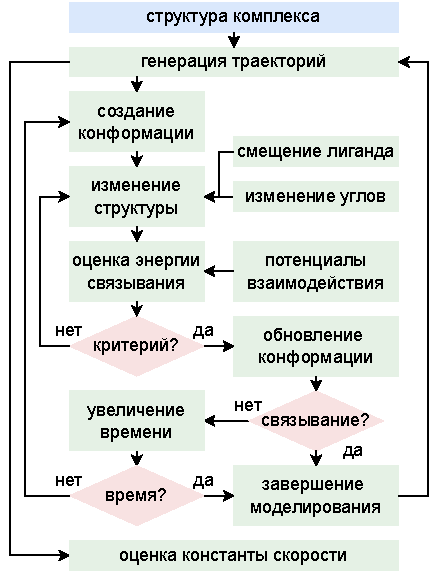
\includegraphics[width=0.39\linewidth]{images/kmc.pdf}
	\caption{Основные этапы работы кинетического метода Монте-Карло}
	\label{monte}
\end{figure}

При этом, поскольку метод является стохастическим, этап оценки взаимодействия повторяется значительное количество раз. В~связи с~этим актуальным становится оптимизация этого этапа без существенной потери качества выполняемых оценок. Следует отметить, что для моделирования процесса образования комплекса достаточно сформировать оценочную функцию, учитывающую только парные межатомные взаимодействия и~влияние растворителя\cite{biom10071056}.

Существует множество инструментов для оценки энергии взаимодействия. Например, выполнить оценку взаимодействия возможно с~помощью фреймворка Rosetta~\cite{rosetta} или силового поля~CHARMM~\cite{brooks}. Следует отметить, что для выполнения оценки требуется представление белкового комплекса внутренними средствами инструмента, что, как правило, довольно накладно с~временной точки зрения. Например, в~случае применения CHARMM перед выполнением оценки требуется перевод структуры во внутренний формат силового поля непосредственно из файла со структурой, а~в~случае применения Rosetta при выполнении оценки происходит обновление энергетической карты, которое также влияет на время выполнения оценки. 

Разработанная в настоящей работе оценочная функция напрямую интегрирована в~библиотеку PSM, что позволяет снизить вычислительную сложность выполнения оценки по сравнению с~использованием внешних инструментов, что подчеркивает актуальность выполненной работы.
